\section{Experimental Configuration}

\subsection{S3 Dataset Details}
Bộ dữ liệu hình ảnh gỗ S3 chứa hình ảnh mặt cắt ngang ở mức vĩ mô (macro) của 19 loài gỗ thuộc 6 chi khác nhau: \textit{Afzelia}, \textit{Dalbergia}, \textit{Guibourtia}, \textit{Peltogyne}, \textit{Pterocarpus} và \textit{Sindora}. Bộ dữ liệu có cấu trúc phân cấp tự nhiên: mỗi loài gỗ tương ứng với một lớp (class); bên trong mỗi loài chứa nhiều thư mục con đại diện cho một mẫu vật lý riêng biệt. Việc giữ nguyên vẹn toàn bộ hình ảnh của cùng một thư mục con vào cùng một tập dữ liệu là bắt buộc để tránh rò rỉ đặc trưng lối tắt từ phiên chụp. Các mẫu gỗ chỉ được định danh ở cấp chi được loại bỏ khỏi quy trình huấn luyện để đảm bảo tính nhất quán của nhãn. Phân bố chi tiết số lượng ảnh và mẫu vật của các tập dữ liệu thành phần sau khi phân chia được minh họa trong Hình \ref{fig:eda_split}.

\begin{figure}[htbp]
\centering
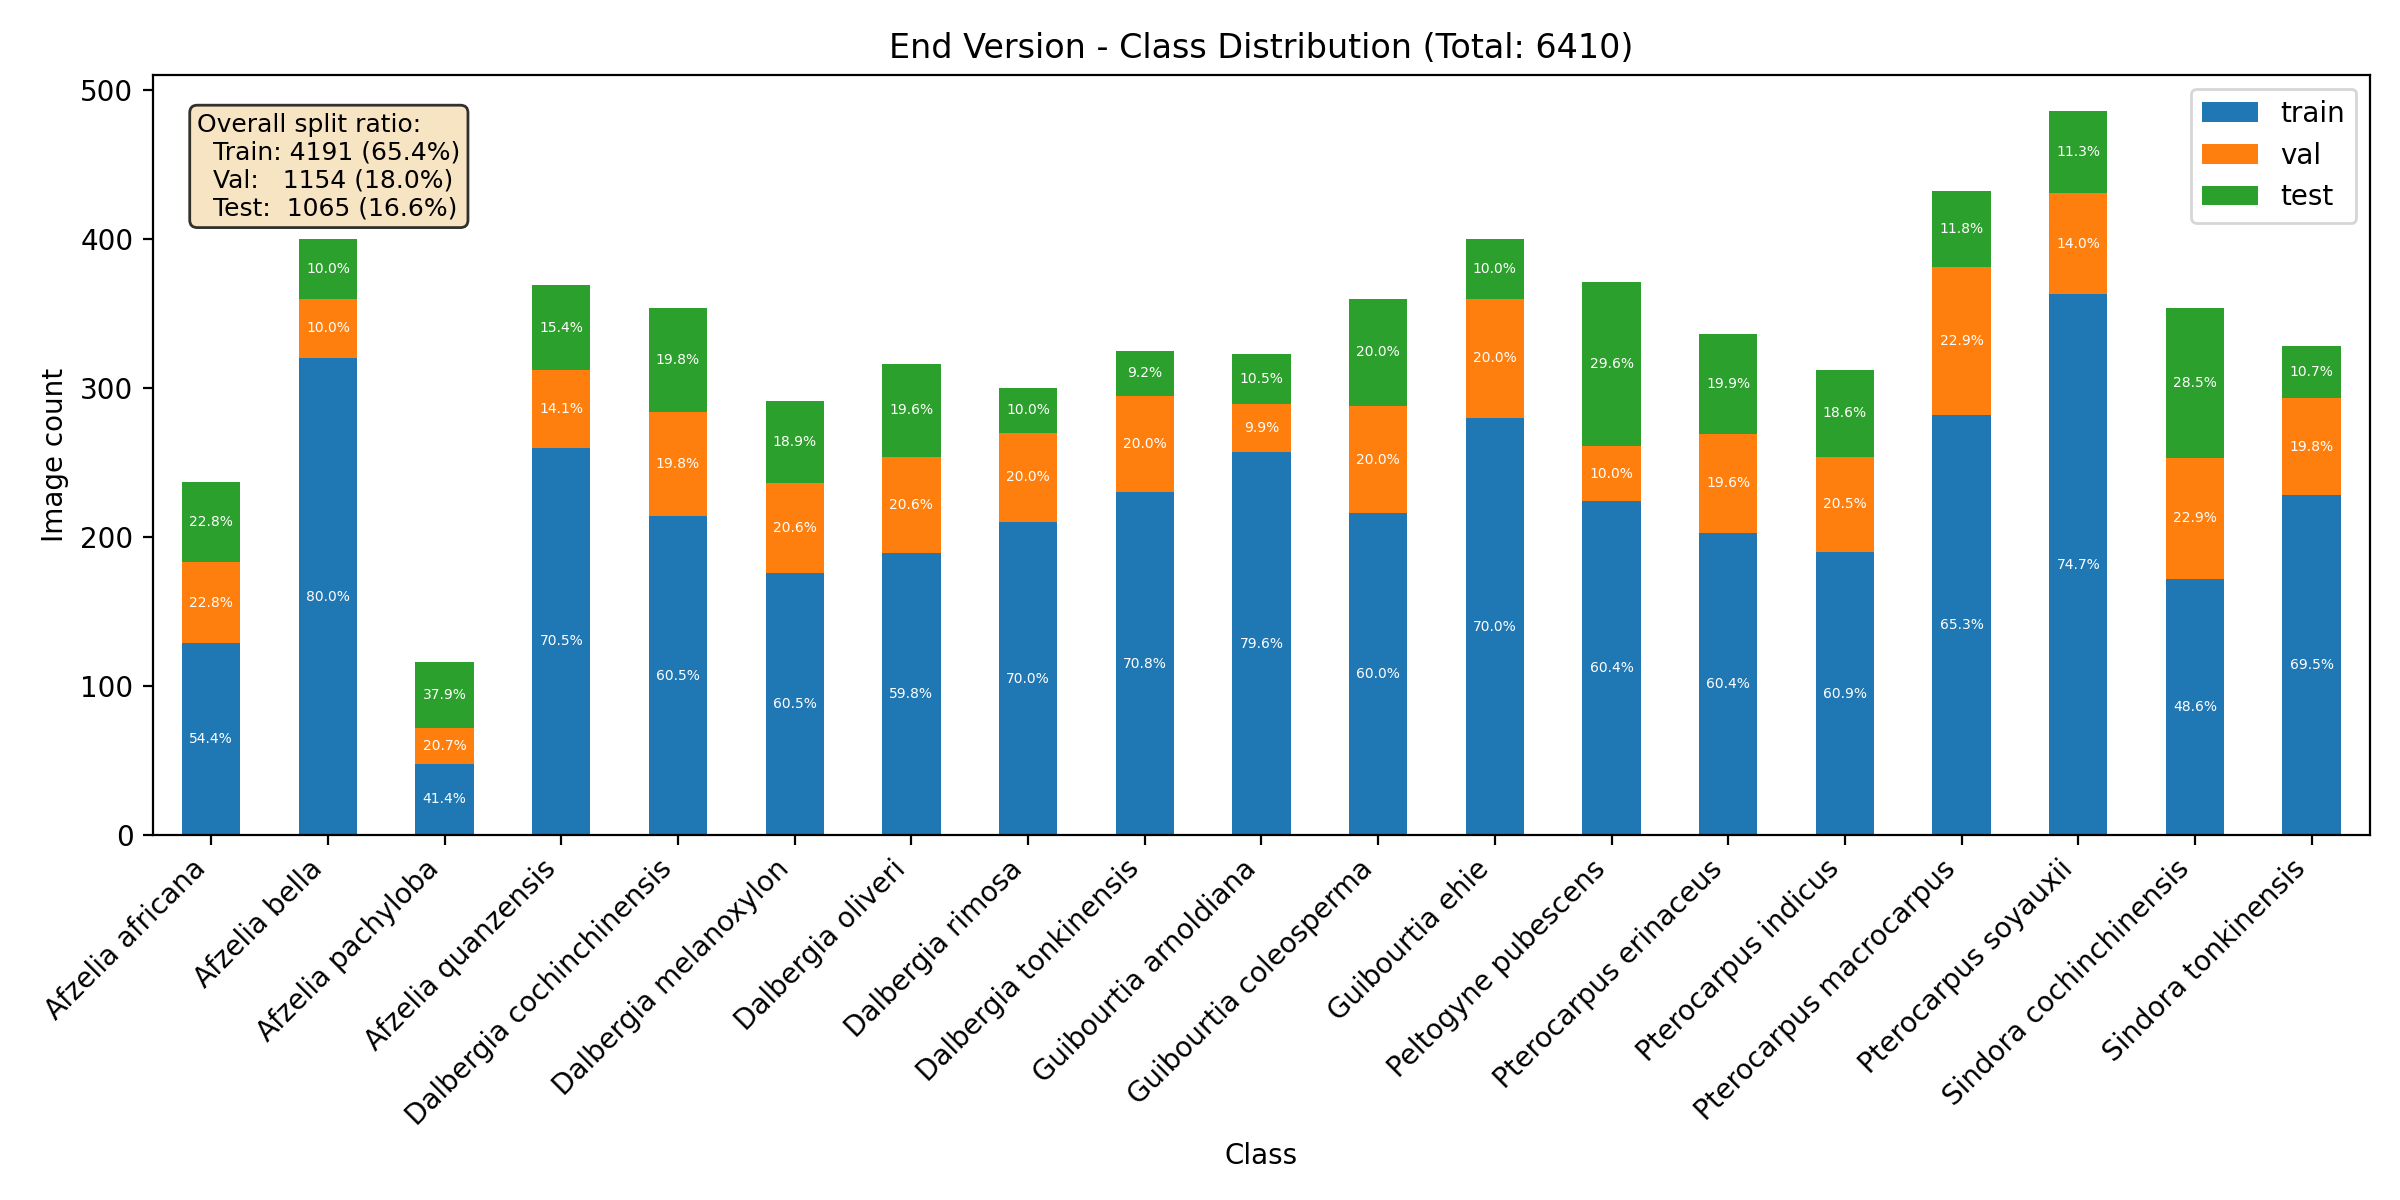
\includegraphics[width=\columnwidth]{fig/eda_split_end_version.png}
\caption{Class-wise specimen and image distribution of the S3 dataset under the CEGS-Split protocol.}
\label{fig:eda_split}
\end{figure}

\subsection{Data Augmentation}
Quy trình tăng cường dữ liệu được thiết kế nhằm bảo toàn các cấu trúc giải phẫu sinh học (vân gỗ, mạch gỗ) nhưng nâng cao khả năng chống chịu trước các biến thiên thực tế: xoay ngẫu nhiên, cắt và thay đổi kích thước (RandomResizedCrop), biến đổi màu sắc nhẹ (ColorJitter), chuyển đổi ảnh xám, làm mờ Gaussian (GaussianBlur), điều chỉnh độ sắc nét và xóa ngẫu nhiên (RandomErasing). Các phép biến đổi này mô phỏng sự khác biệt về hướng cắt, độ phóng đại ống kính, độ sáng và các yếu tố nhiễu bề mặt.

\subsection{Benchmarking Protocols}
Nghiên cứu tiến hành đánh giá thực nghiệm đối chiếu 14 phương pháp học khoảng cách: Triplet cơ bản, Triplet bán khó, Triplet biên mềm, Angular, Multi-Similarity, Contrastive cơ bản, Contrastive khai thác cặp khó, Lifted Structured, Circle, Proxy Anchor, ArcFace, SubCenter ArcFace, SoftTriple và tương phản có giám sát (SupCon). Nhóm tự giám sát bao gồm bốn mô hình: SimCLR, BYOL, SimSiam và Barlow Twins. Tất cả các phương pháp này đều được huấn luyện và kiểm thử trên cùng một cấu hình chia dữ liệu thu được từ giao thức CEGS-Split để đảm bảo tính khách quan và loại trừ các sai số do phân bổ dữ liệu.

\subsection{Embedding Space Evaluation Metrics}
Chất lượng của không gian nhúng biểu diễn đặc trưng được kiểm chứng qua hai nhóm chỉ số đo lường chính. Nhóm truy xuất (retrieval) bao gồm: Recall@k, Precision@k, mAP và AUC. Đối với từng chỉ số đo lường theo từng lớp $x_i$, báo cáo sử dụng cả giá trị macro average (macro average) và harmonic mean (harmonic mean) kèm theo một ngưỡng làm mịn $\epsilon=0.01$ để tránh chia cho 0:
\begin{equation}
\text{HM}=\frac{N}{\sum_{i=1}^{N}\frac{1}{x_i+\epsilon}},\quad \epsilon=0.01.
\end{equation}
Chỉ số harmonic mean (Harmonic mean) giúp phản ánh chính xác hiệu năng ở các lớp gỗ yếu, tránh tình trạng mô hình đạt điểm số macro average (macro average) cao nhờ các loài dễ phân biệt nhưng lại hoàn toàn thất bại ở các loài gỗ cùng chi có độ tương đồng hình thái cao (fine-grained).

Nhóm clustering gồm Silhouette Score, Davies-Bouldin Index, Calinski-Harabasz Index, Dunn Index và Normalized Mutual Information. Với một mẫu $i$, Silhouette được tính:
\begin{equation}
s(i)=\frac{b(i)-a(i)}{\max(a(i),b(i))},
\end{equation}
trong đó $a(i)$ là khoảng cách trung bình đến các mẫu cùng cụm và $b(i)$ là khoảng cách trung bình nhỏ nhất đến cụm khác. Davies-Bouldin Index là
\begin{equation}
\text{DBI}=\frac{1}{C}\sum_{i=1}^{C}\max_{j\ne i}\frac{\sigma_i+\sigma_j}{d(\mu_i,\mu_j)}.
\end{equation}
Dunn Index được định nghĩa:
\begin{equation}
\text{DI}=\frac{\min_{i\ne j}\delta(C_i,C_j)}{\max_k\Delta(C_k)}.
\end{equation}
NMI đo mức tương đồng thông tin giữa nhãn cụm dự đoán và nhãn loài thật:
\begin{equation}
\text{NMI}(Y,C)=\frac{2I(Y;C)}{H(Y)+H(C)}.
\end{equation}

\subsection{Implementation Hyperparameters}
Mô hình được tối ưu hóa bằng thuật toán AdamW với tốc độ học (learning rate) $10^{-4}$ và hệ số suy giảm trọng số (weight decay) $10^{-2}$. Bộ lập lịch suy giảm tốc độ học theo hàm cosin (Cosine Annealing scheduler) được sử dụng trong tối đa 100 chu kỳ huấn luyện (epoch). Cơ chế dừng sớm (early stopping) giám sát chỉ số harmonic mAP trên tập kiểm định với ngưỡng chờ (patience) là 30 chu kỳ. Số chiều đặc trưng nhúng (embedding dimension) mặc định là 256, tỷ lệ đóng băng các lớp mạng (freeze ratio) mặc định là $90\%$, và mạng cơ sở (backbone) chính được sử dụng là ConvNeXt-Tiny. Các thực nghiệm loại bỏ thành phần (ablation study) được thiết kế chi tiết để đánh giá ảnh hưởng của cấu trúc mạng cơ sở, số chiều đặc trưng nhúng, tỷ lệ đóng băng lớp mạng, phương pháp phân chia dữ liệu và hàm loss.

